\section{Introduction}
\begin{wrapfigure}{r}{0.4\textwidth}
  \begin{center}
    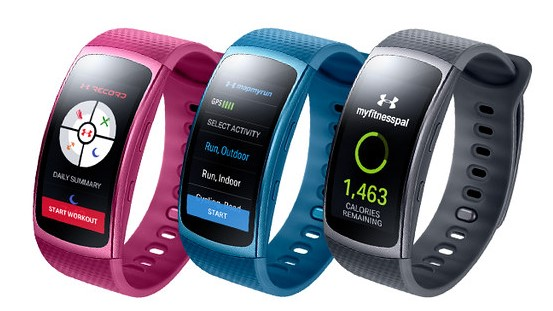
\includegraphics[width=0.4\textwidth]{assets/SamsungWearables.jpg}
  \end{center}
  \caption{Fitness Wearables from Samsung Electronics and Under Armour}
  \label{fig:SamsungWearables}
\end{wrapfigure}
In today's mesmerizing technological front, fitness devices are neither a sci-fi dream nor an archaic fad. Wearable devices that provide quantitative analyses of the wearer's health have struck the market as an exoskeletal element of the Internet of Things \cite{ref05}, and they improve in quality and quantity with every release. However, despite their popularity and success, there remains the vital need to examine if these devices are really useful and how far they have gotten.

To answer these critical questions, we analyze the results of three research studies that investigate the effects of using fitness trackers, steps counters, etc. on the health and well-being of individuals. The first \cite{ref01} is a systematic review and network meta-analysis that was conducted at the School of Kinesiology, University of Minnesota Twin Cities, Minneapolis. On the other hand, the second study \cite{ref02} is a randomized clinical trial that was conducted at the University of Pittsburgh. Finally, the third study \cite{ref03} at the Anschutz Medical Campus, University of Colorado, involves a systematic review of studies that engaged people in the use of smart watches. These studies help us analyze the popularity of wearable fitness devices as well as their impacts on the health lifestyle of the users.